% Preamble
\documentclass{beamer}
\usepackage[utf8]{inputenc}
\usepackage{german}
\usepackage{ngerman}
\usepackage{tikz}
\usepackage{pgfplots}
\usepackage{eurosym}
\usepackage{amsmath}

\title[TSP]
{Travelling Salesman Problem}
\subtitle{Exakte Lösungen}
\author
{Axel Christ}
\institute{DHBW Karlsruhe}
\subject{Theorieseminar Informatik}

\AtBeginSection[]
{
  \begin{frame}
    \frametitle{Table of Contents}
    \tableofcontents[currentsection]
  \end{frame}
}

\begin{document}
  \frame{\titlepage}
  \section{Definition}
  \begin{frame}
    \frametitle{Definition}
    Ein Handlungsreisender muss mehrere Städte besuchen. Dabei soll die
    Strecke, um alle Städte zu besuchen, möglichst kurz sein.
    \pause
    \begin{figure}
      \centering
      \includegraphics[width=\linewidth,height=150px,keepaspectratio]{alltag.png}
      \caption{Alltag für Viele}
    \end{figure}
  \end{frame}

  \begin{frame}
    \frametitle{Definition}
    Es gibt $N$ Städte.
    Zwischen zwei Städten $i$ und $j$ gibt es jeweils eine Kante $c_{ij}$.
    Sollte einmal keine Kante bestehen, so wird eine Kante mit großer Länge
    automatisch eingefügt.
  \end{frame}

  \begin{frame}
    \frametitle{TSP-Klassifikationen}
    \begin{itemize}[<+->]
      \item \textbf{Symmetrisches TSP}
        \linebreak
        Ungerichteter Graph
        $$c_{ij} = c_{ji}$$
        Hin- und Rückweg zwischen zwei Knotenpunkten stets gleich
      \item \textbf{Asymmetrisches TSP}
        \linebreak
        Gerichteter Graph
        Hin- und Rückweg zwischen zwei Knotenpunkten muss nicht gleich sein
      \item \textbf{Metrisches TSP}
        \linebreak
        Erfüllen der Dreiecksungleichung
        $$c_{ij} \le c_{ik} + c_{kj}$$
        Verbindung von $i$ nach $j$ nie länger als über dritten Knoten $k$
    \end{itemize}
  \end{frame}

  \begin{frame}
    \frametitle{Nicht-metrisches TSP}
    Ein TSP-Problem kann auch nicht-metrisch sein, wenn Umrüstzeiten
    berücksichtigt werden müssen.
    \pause
    \linebreak
    Beispiel: Drei Trucks sollen an verschiedenen Stationen Gegenstände
    abliefern und aufnehmen:
    \begin{figure}
      \centering
      \includegraphics[width=\linewidth,height=150px,keepaspectratio]{truck_problem.png}
      \caption{Truck Problem}
    \end{figure}
  \end{frame}

  \section{Komplexität}
  \begin{frame}
    \frametitle{Komplexitätsbetrachtung}
    Bei einem symmetrischen TSP gibt es $\frac{(n-1)!}{2}$ mögliche Routen,
    bei einem asymmetrischen $(n-1)!$ mögliche!

    \newcount\mycount

    \begin{figure}
      \centering
      \begin{tikzpicture}[transform shape,scale=0.4]
        %the multiplication with floats is not possible. Thus I split the loop in two.
        \foreach \number in {1,...,8}{
            % Computer angle:
              \mycount=\number
              \advance\mycount by -1
        \multiply\mycount by 45
              \advance\mycount by 0
            \node[draw,circle,inner sep=0.25cm] (N-\number) at (\the\mycount:5.4cm) {};
          }
        \foreach \number in {9,...,16}{
            % Computer angle:
              \mycount=\number
              \advance\mycount by -1
        \multiply\mycount by 45
              \advance\mycount by 22.5
            \node[draw,circle,inner sep=0.25cm] (N-\number) at (\the\mycount:5.4cm) {};
          }
        \foreach \number in {1,...,15}{
              \mycount=\number
              \advance\mycount by 1
        \foreach \numbera in {\the\mycount,...,16}{
          \path (N-\number) edge[->,bend right=3] (N-\numbera)  edge[<-,bend
            left=3] (N-\numbera);
        }
      }
      \end{tikzpicture}
      \caption{Anzahl mögliche Verbindungen bei $n=16$}
    \end{figure}
  \end{frame}

  \section{Exakte Lösungen}

  \begin{frame}
    \frametitle{Lösung durch Permutation}

    \begin{enumerate}[<+->]
      \item Permutation durch alle möglichen Touren
      \item Für kleine $n$ noch machbar
      \item Jedoch: $n$ steigt schnell drastisch an (Fakultät)
    \end{enumerate}

    \begin{figure}
      \centering
      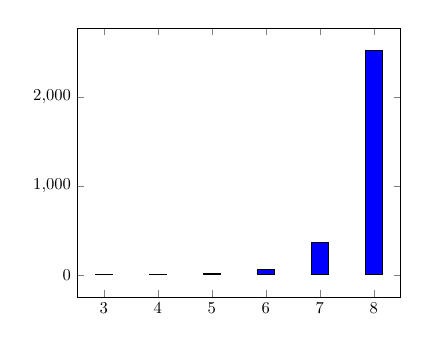
\begin{tikzpicture}[scale=0.6]
        \begin{axis}[
            symbolic x coords={3, 4, 5, 6, 7, 8},
            xtick=data
          ]
            \addplot[ybar,fill=blue] coordinates {
                (3, 1)
                (4, 3)
                (5, 12)
                (6, 60)
                (7, 360)
                (8, 2520)
            };
        \end{axis}
      \end{tikzpicture}
      \caption{Anzahl Touren in Abhängigkeit $n$ bei symmetrischem TSP}
    \end{figure}
  \end{frame}

  \subsection{Lineare Programmierung}
  \begin{frame}
    \frametitle{Problemstellung}

    Eine Möbelfirma produziert zwei Arten von Sofas: Ein Standard-
    und ein Sondermodell.
    \pause
    \\~\\

    Die Produktion eines Standardmodells benötigt zwei Stunden, die
    eines Sondermodells drei.
    \pause
    \\~\\

    Drei Arbeiter arbeiten jew. 8 Stunden am Tag
    \pause
    \\~\\

    Der maximale tägliche Bedarf an Standardsofas ist 6, bei
    Sondersofas 8.
    \pause
    \\~\\

    Ein Standardsofa bringt 500\euro, ein Sondermodell 300\euro.
    \pause
    \\~\\

    \textbf{Wie kann der Profit der Möbelfirma maximiert werden?}
  \end{frame}

  \begin{frame}
    \frametitle{Datenanalyse}

    \textbf{Was sind die Entscheidungsvariablen?}
    \linebreak
    \pause
    Anzahl der Standardsofas ($x$) und Anzahl der Sondersofas ($y$) die pro
    Tag produziert werden sollen.
    \pause
    \\~\\

    \textbf{Was sind die Randbedingungen?}
    \pause
    \begin{itemize}[<+->]
      \item Verfügbare Arbeitskapazität pro Tag: $3 \cdot 8 = 24$
      \item Maximale Nachfrage pro Tag
        \begin{itemize}
          \item Standardsofas: 6
          \item Sondersofas: 8 
        \end{itemize}
      \item Zeitverbrauch pro Einheit
        \begin{itemize}
          \item Standardsofa: 2h
          \item Sondersofa: 3h 
        \end{itemize}
    \end{itemize}
  \end{frame}

  \begin{frame}
    \frametitle{Mathematische Repräsentation}

    \textbf{Zielfunktion}
    $$f(x) = 500x \cdot 300y $$
    \pause

    \textbf{Nachfrage}
    $$x \leq 6$$
    $$y \leq 8$$
    \pause

    \textbf{Max. Arbeitskapazität}
    $$2x + 3y \leq 24$$
    \pause

    \textbf{Entscheidungsvariablen müssen nichtnegativ sein}
    $$x, y \geq 0$$
  \end{frame}

  \begin{tikzpicture}
    \begin{axis}[
      title=Optimierungsproblem
      xlabel={$x$}
      ylabel={$y$}
    ]

    \addplot{exp(2*x + 3*y)};
      
    \end{axis}
  \end{tikzpicture}

\end{document}